% вторая часть

\section{Примеры использования элементов текста}

В данном разделе приводятся примеры добавления в текст элементов, которые могут нумероваться автоматически --- таблиц, рисунков, листингов программ. Важно запомнить, что для корректной работы с такими элементами следует задавать их названия командой \Verb|\caption{название}| и определять символическое имя (метку) командой \Verb|\label{ключ}|. По этому ключу можно ссылаться на соответствующий объект в тексте командой \Verb|\ref{ключ}|, см. примеры ниже.

\subsection{Рисунки}

Для добавления нумерованного рисунка следует использовать окружение figure. Пример приведен на рис.~\ref{fig:ris1}.

\begin{figure}[H]
\centering
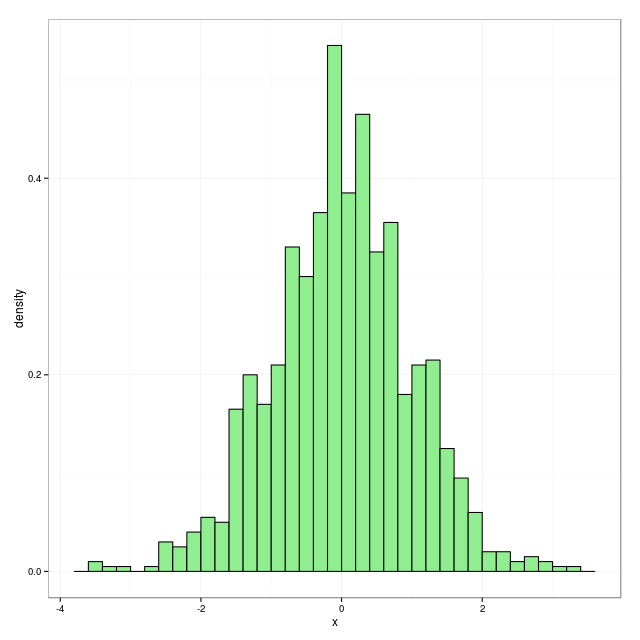
\includegraphics[width=0.5\linewidth]{pics/ris1} % изображения хранятся в подкаталоге pics
\caption{Пример добавления графики как нумерованного рисунка}
\label{fig:ris1} % эта метка позволяет ссылаться на рисунок в тексте
\end{figure}

График построен с использованием языка программирования \textbf{R} \cite{RManual}.

\subsection{Таблицы}

Таблицы добавляются в текст аналогично графике, только используется окружение table (см. таблицу~\ref{tab:tab1}).

\begin{table}[H]
\caption{Заполнение ячеек} \label{tab:tab1}
\centering
\begin{tabular}{|c|c|c|c|}
\hline 1 & a & b & c \\ 
\hline  2 & Строка 1 &Пример 1  & Дополнительно \\ 
\hline 3 &  Строка 2&  Пример 2&  \\ 
\hline 
\end{tabular} 
\end{table}

\subsection{Исходный код}

Исходный код программ можно добавить с помощью окружений, определенных сразу после преамбулы. Пример --- на листинге~\ref{lst:1}.


\begin{flushleft}
\needspace{3\baselineskip}
\captionof{Program}{Пример кода на языке R} \label{lst:1}
\begin{MyCodes}
# Проверка и тестирование пакета deSolve
require(deSolve)
require(rgl)

# система Хиндмарша - Розе с параметрами
# используются параметры в виде списка (parms$a etc)
hindrose <- function(t,y,parms)
{
 ydot <- vector(len=3)
 ydot[1] <- y[2] - parms$a * y[1]^3 + parms$b*y[1]^2 + parms$Iext - y[3]
 ydot[2] <- parms$c - parms$d*y[1]^2 - y[2]
 ydot[3] <- parms$r * (parms$s*(y[1]-parms$xs)-y[3])
 return(list(ydot))
}
\end{MyCodes}
\end{flushleft}